\documentclass[tikz,border=6pt]{standalone}
\usepackage{pgfplots}\pgfplotsset{compat=1.16}
\usetikzlibrary{arrows.meta,decorations.markings}
\definecolor{red}{HTML}{A50F2D}\definecolor{ink}{HTML}{141414}\definecolor{gry}{HTML}{5F5F5F}
\begin{document}
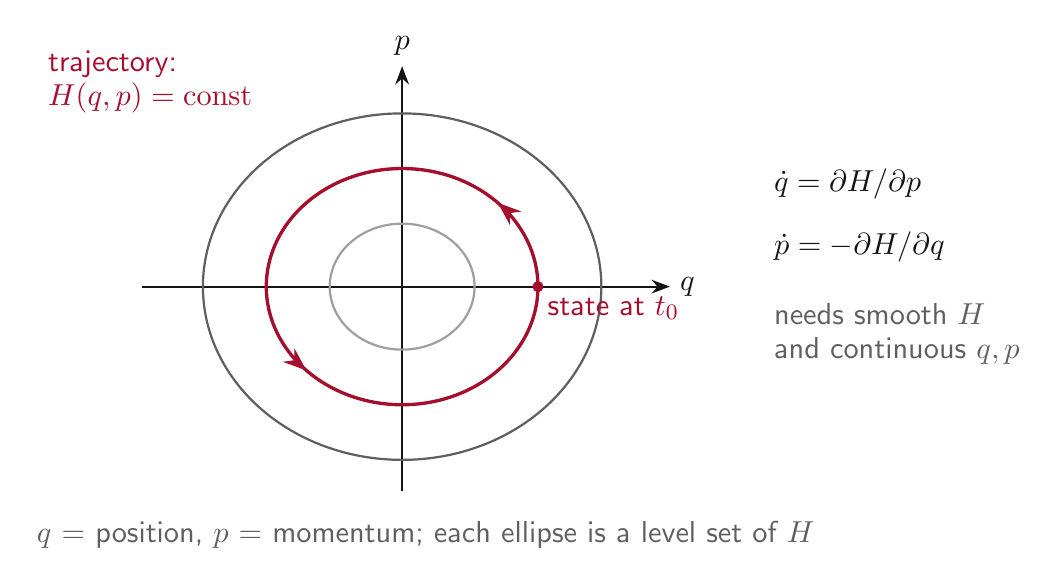
\begin{tikzpicture}[font=\sffamily\fontsize{11}{13}\selectfont,>=Stealth]
% axes
\draw[->,ink,thick] (-3.3,0)--(3.4,0) node[right]{$q$};
\draw[->,ink,thick] (0,-2.6)--(0,2.8) node[above]{$p$};
% level sets of H = p^2/2 + q^2/2 (ellipses)
\foreach \r/\c in {0.8/gry!60,1.5/gry!80,2.2/gry}{
  \draw[\c,thick] (0,0) ellipse ({\r*1.15} and {\r});}
% trajectory
\draw[red,very thick,
  postaction={decorate,decoration={markings,mark=at position 0.12 with {\arrow{Stealth}},mark=at position 0.62 with {\arrow{Stealth}}}}]
  (0,0) ellipse (1.725 and 1.5);
\fill[red] (1.725,0) circle (2pt) node[below right,red]{state at $t_0$};
\node[red,align=left] at (-3.2,2.6) {trajectory:\\[-1pt]$H(q,p)=\mathrm{const}$};
\node[gry,align=center] at (0.3,-3.15) {$q$ = position, $p$ = momentum; each ellipse is a level set of $H$};
\node[ink,align=left,anchor=west] at (4.6,1.3) {$\dot q = \partial H/\partial p$};
\node[ink,align=left,anchor=west] at (4.6,0.5) {$\dot p = -\partial H/\partial q$};
\node[gry,align=left,anchor=west] at (4.6,-0.6) {needs smooth $H$\\[-1pt]and continuous $q,p$};
\end{tikzpicture}
\end{document}
